\documentclass[../Funzionalita.tex]{subfiles}

\begin{document}

\subsection{Navigazione}
\label{subsec:Navigazione}

		\subsubsection{Panoramica}
			La funzionalità di navigazione è resa disponibile dalle componenti dei package:
			\begin{itemize}
				\item \navigator;
				\item \beacon;
				\item \compass;
				\item \dataaccess;
				\item \usersetting.
			\end{itemize}
			Esse permettono di guidare l'utente all'interno di un edificio.
			La navigazione è gestita attraverso queste fasi:
			\begin{enumerate}
				\item l'utente interagendo con l'interfaccia grafica avvia la navigazione;
				\item la business logic dell'applicazione costruisce un grafo;
				\item alle componenti di \navigator\ viene passato il grafo;
				\item viene calcolato il percorso utilizzando la libreria esterna \textbf{JgraphT};
				\item vengono restituite le informazioni necessarie per guidare l'utente verso la destinazione da lui scelta;
				\item l'interfaccia mostra all'utente le informazioni.
			\end{enumerate}
			
		\newpage
		\subsubsection{Interfaccia grafica}
			La navigazione comprende diverse viste. Tutto parte dalla vista della \HomeView\ da cui è possibile selezionare la categoria della possibile destinazione, formalmente descritta come \textit{point of interest} (POI). Una volta selezionata la categoria l'utente passa alla vista \PoiCategoryViewImp\ che mostra  la lista di possibili destinazioni della categoria selezionata. Una volta selezionata la destinazione all'utente è mostrata una nuova vista che presenta tutti i passaggi necessari per raggiungerla. \NavigationView\ e \PoiCategoryView\ sono rispettivamente collegate alle classi che rappresentano il presenter \NavigationActivity\ e \PoiCategoryActivity.
			
			\paragraph*{Componenti interne}
			\begin{itemize}
			
				\item Package:
				\begin{itemize}
					\item[] \view;
				\end{itemize}
				
				\item Interfacce e classi:
				\begin{itemize}
					\item[] \PoiCategoryView, \PoiCategoryViewImp, \NavigationView, \NavigationViewImp;
				\end{itemize}
				
			\end{itemize}
			
			
			\paragraph*{Componenti esterne}
			\begin{itemize}
				\item Interfacce e classi SDK:
				\begin{itemize}
					\item[] \AdapterView, \ArrayAdapter, \ListView;
				\end{itemize}
			\end{itemize}
			
			Nella figura \ref{fig:Navigazione-NavigationView} si indicano i seguenti widget offerti dal kit \gls{Android} SDK :
			\begin{enumerate}
				\item \Toolbar;
				\item \ListView.
			\end{enumerate}
		
		\newpage	
		\vfill
			\begin{figure} [h]
				\centering
				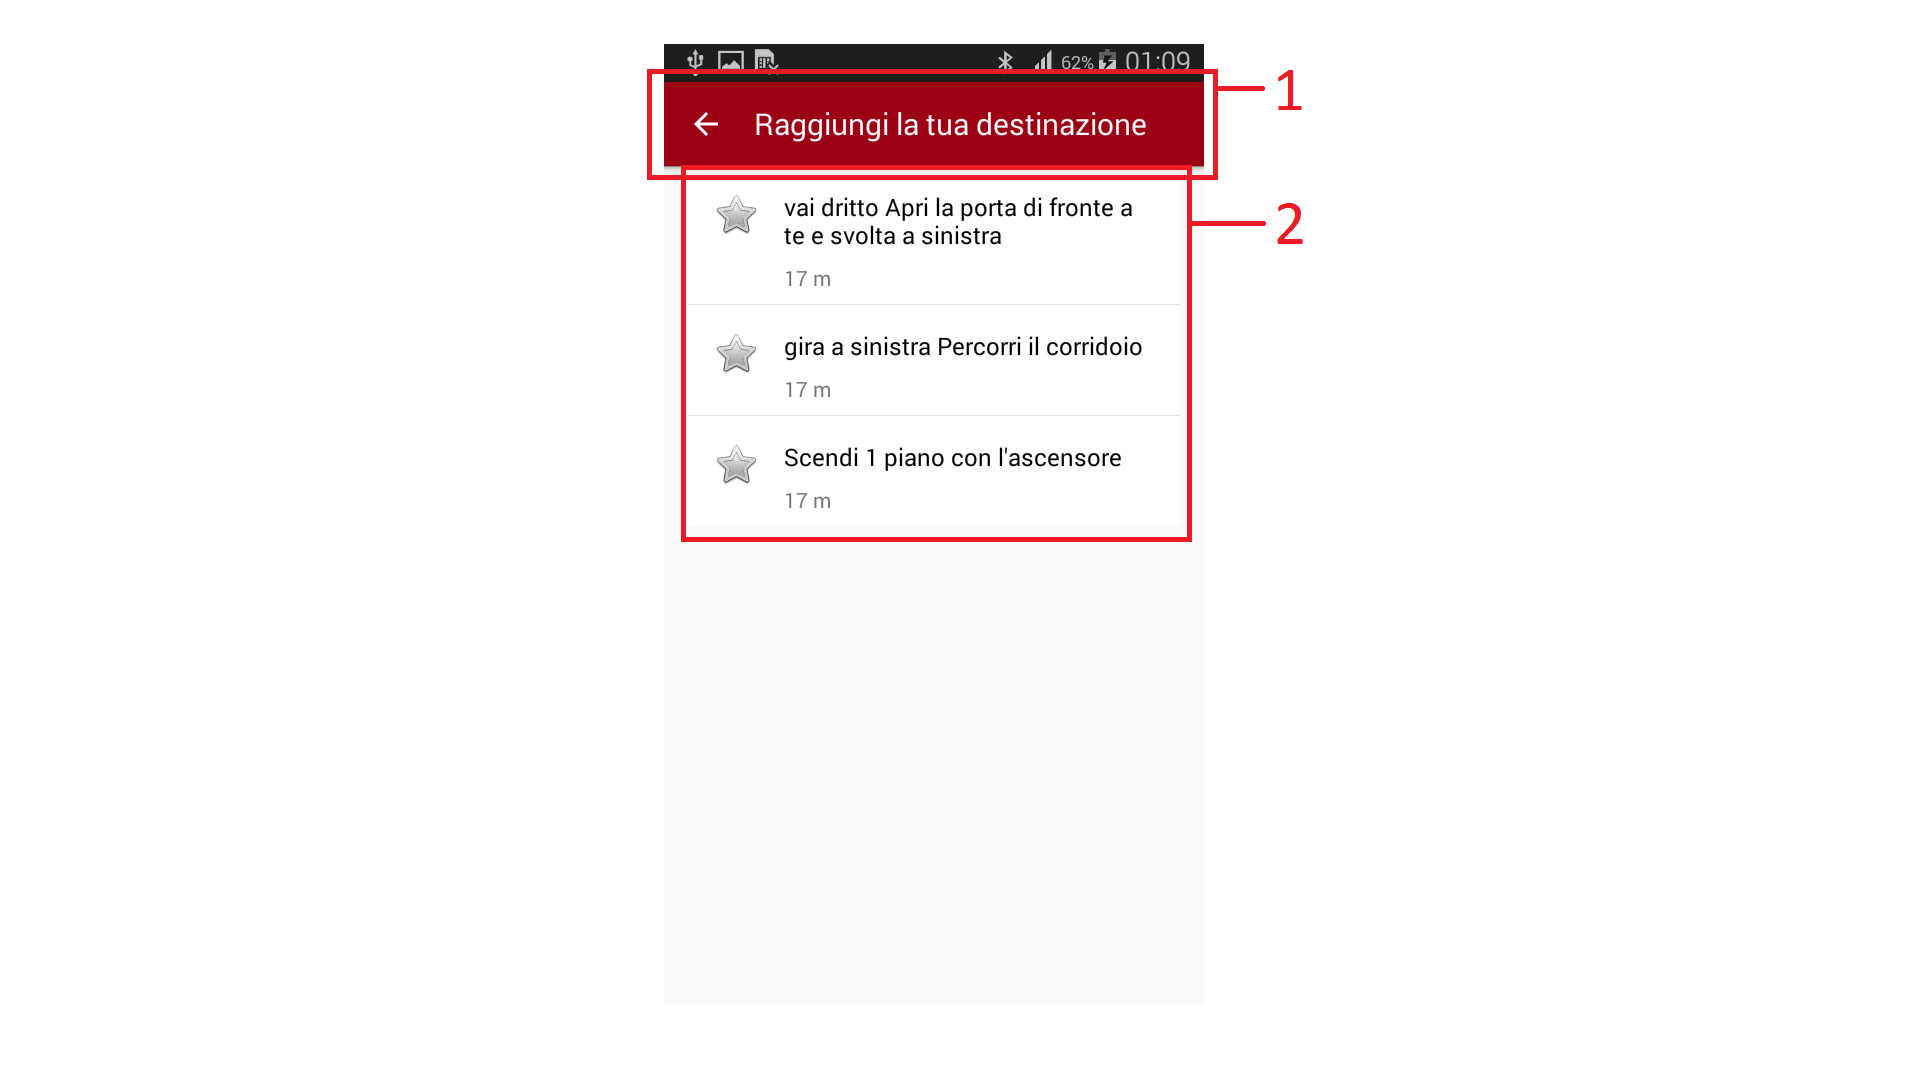
\includegraphics[width=\textwidth]{img/Navigazione-NavigationView_}
				\caption{Navigazione - Lista istruzioni percorso}
				\label{fig:Navigazione-NavigationView}
			\end{figure}
			\vfill
			\begin{figure} [h]
				\centering
				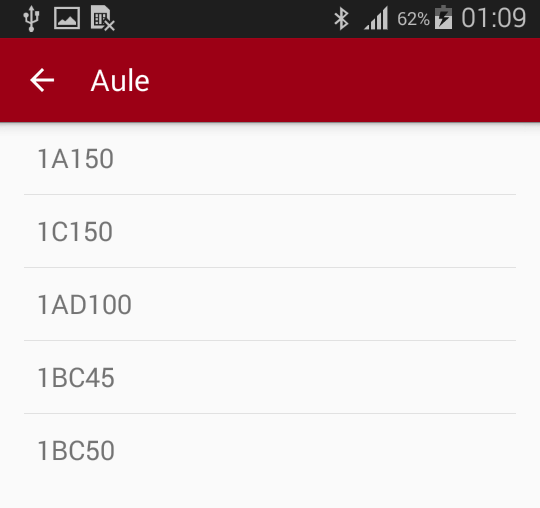
\includegraphics[scale=0.3]{img/Navigazione-PoiCategoryView_}
				\caption{Navigazione - Scelta destinazione nella categoria \textit{Aule}}
				\label{fig:Navigazione-PoiCategoryView}
			\end{figure}
		\vfill
		
		
		\newpage
		\subsubsection{Presenter}
			Il compito del presenter per questa funzionalità è affidato all'oggetto \PoiCategoryActivity\ che comunica con la vista \PoiCategoryViewImp\ attraverso l'interfaccia \HomeView\ e \NavigationActivity\ che comunica con la vista \NavigationViewImp\ attraverso l'interfaccia \NavigationView. \PoiCategoryActivity\ comunica con le componenti del model \InformationManager\ attraverso la dependency injection mentre \NavigationActivity\ comunica con le componenti del model \InformationManager\ e \NavigationManager\ sempre attraverso l'uso della dependency injection.
		
			\paragraph*{Componenti interne}
			\begin{itemize}
			
				\item Package:
				\begin{itemize}
					\item[] \view;
					\item[] \presenter;
				\end{itemize}
				
				\item Interfacce e classi:
				\begin{itemize}
					\item[] \NavigationActivity, \PoiCategoryActivity, \NavigationView, \PoiCategoryView, \NavigationAdapter;
				\end{itemize}
				
			\end{itemize}
			
			
			\paragraph*{Componenti esterne}
			
			\begin{itemize}
				\item Interfacce e classi SDK:
				\begin{itemize}
					\item[] \Activity, \AppCompatActivity;
				\end{itemize}
			\end{itemize}
					
		
		\subsubsection{Calcolo percorso}
			La classe \NavigationManagerImp\ richiede il calcolo del percorso a \Navigator\ implementata dalla classe \NavigatorImp. Affinché \NavigatorImp\ funzioni devono essere effettuate alcune operazioni nel giusto ordine qui riportato (\textbf{nota:} non vengono riportati i parametri, per essi si faccia riferimento alla javadoc):
			\begin{enumerate}
				\item eseguire la chiamata del metodo \lstinline|setGraph()| settare il grafo dell'edificio rilevato;
				\item eseguire la chiamata del metodo \lstinline|calculatePath()| per far sì che \NavigatorImp\ calcoli il percorso dal punto in cui si è (\lstinline|startROI|) alla destinazione scelta (\lstinline|endPOI|)
				\item utilizzare uno o entrambi i metodi che ritornano informazioni incapsulate in \ProcessedInformation:
				\begin{itemize}
					\item \lstinline|getAllInstruction()| per recuperare immediatamente tutte le informazioni per raggiungere la destinazione;
					\item \lstinline|toNextRegion()| per recuperare solo l'informazione del prossimo punto da raggiungere, guidando l'utente con un passaggio alla volta.
				\end{itemize}
			\end{enumerate}
		
			\paragraph*{Componenti interne}
			\begin{itemize}
			
				\item Package:
				\begin{itemize}
					\item[] \navigator;
					\item[] \algorithm;
					\item[] \graph;
					\item[] \area;
				\end{itemize}
				
				\item Interfacce e classi:
				\begin{itemize}
					\item[] \Navigator, \NavigatorImp, \ProcessedInformation, \ProcessedInformationImp, \PathFinder, \DijkstraPathFinder, \Compass, \MapGraph, \EnrichedEdge, \PointOfInterest, \RegionOfInterest;
				\end{itemize}
				
			\end{itemize}
			
			
			\paragraph*{Componenti esterne}
			
			\begin{itemize}
				\item Interfacce e classi JGraphT:
				\begin{itemize}
					\item[] \DijkstraShorterPath, \SimpleDirectedWeightedGraph.
				\end{itemize}
			\end{itemize}
		
		
		\subsubsection{Bussola}
			La classe \Compass\ permette all'applicazione di ricevere dati dai sensori hardware del device gestiti grazie alla classe \Sensor. \Compass\ rende disponibili i metodi per registrare i listener ai sensori e per disattivarli. Poiché i sensori comunicano attraverso eventi tramite interfaccia \SensorEventListener\ i dati vengono segnalati in tempo reale direttamente alle classi che implementeranno \CompassListener, tra questi c'è \NavigationActivity.
		
			\paragraph*{Componenti interne}
			\begin{itemize}
			
				\item Package:
				\begin{itemize}
					\item[] \compass;
				\end{itemize}
				
				\item Interfacce e classi:
				\begin{itemize}
					\item[] \Compass, \CompassListener;
				\end{itemize}
				
			\end{itemize}
			
			
			\paragraph*{Componenti esterne}
			\begin{itemize}
			
				\item Interfacce e classi SDK:
				\begin{itemize}
					\item[] \SensorManager, \Sensor, \SensorEventListener.
				\end{itemize}
				
			\end{itemize}
						
			
		\subsubsection{Eccezioni e gestione}
		\paragraph*{Componenti interne}
			\begin{itemize}
			
				\item Package:
				\begin{itemize}
					\item[] \model;
					\item[] \navigator;
				\end{itemize}
				
				\item Interfacce e classi:
				\begin{itemize}
					\item[] \NavigationManagerImp, \Navigator, \NavigatorImp, \NavigationExceptions, \NoGraphSetException, \PathException, \NoNavigationInformationException;
				\end{itemize}
				
			\end{itemize}
			
			
			\paragraph*{Componenti esterne}
			\begin{itemize}
			
				\item Interfacce e classi JDK:
				\begin{itemize}
					\item[] \Exception.
				\end{itemize}
				
			\end{itemize}
			
			Nel package \navigator\ vengono lanciate delle eccezioni per far sì che chiunque le utilizzi rispetti un particolare ordine. Tale ordine coinvolge le seguenti operazioni:
			\begin{itemize}
				\item Set del grafo in \NavigatorImp;
				\item Calcolo del percorso attraverso \NavigatorImp;
				\item Esecuzione della navigazione.
			\end{itemize}
			Il non rispetto di tale ordine può sollevare diversi tipi di eccezioni:
			\begin{itemize}
				\item \NoGraphSetException\ se il grafo non è stato settato e si richiede il calcolo del percorso o l'esecuzione della navigazione;
				\item \NoNavigationInformationException\ se si avvia la navigazione ma non si è calcolato il percorso precedentemente.
			\end{itemize}
			Mentre se il rilevamento dei \gls{beacon} non corrisponde con quanto previsto, a significare che l'utente sta sbagliando percorso, viene lanciata l'eccezione:
			\begin{itemize}
				\item \PathException.
			\end{itemize}
			Nell'applicazione tali operazioni sono gestite da \NavigationManagerImp.

\end{document}